
\chapter{Binary Translation}
\label{ch-bintrans}

{\small
\begin{flushright}
Design: Cristina, Norman; Documentation: Cristina [c.1996]
\end{flushright} 
}


Binary translation, the process of translating binary executables\footnote{
In this document, the terms \emph{binary executable}, \texttt{executable},
and \texttt{binary} are used as synonyms to refer to the binary image
file generated by a compiler or assembler to run on a particular 
computer.
} makes it possible to run code compiled for source
platform M$_s$ on destination platform M$_d$.  Unlike an interpreter or
emulator, a binary translator makes it possible to approach the speed
of native code on machine M$_d$.  Translated code may run more slowly than
native code because low-level properties of machine M$_s$ must often be
modeled on machine M$_d$.  For example, the Digital Freeport Express
translator~\cite{Dec95} simulates the byte order of SPARC, and the FX!32 
translator~\cite{Thom96,Hook97} simulates the calling sequence of the 
source x86 machine, even though neither of these is native to the target 
Alpha.

Because code for decoding, analyzing, translating, and emitting
machine instructions is highly machine-dependent and is written by
hand, existing binary translators are limited to one or two platforms.
Our research makes it much easier to build binary translators for new 
platforms.  It also lays a foundation for the development of new analyses 
that could improve the performance of translated code; for example, it 
might be possible to use native byte order or calling sequences in 
many cases.

Commercial hardware and software companies (e.g. Digital, AT\&T, Sun) 
have invested significant resources in the development of
automatic binary translation, but some of the approaches have been
constrained by time-to-market issues.  Our research attacks  
problems that cannot be considered in a product setting scenario.


\section{Is Binary Translation the Solution to all Migration Problems?}
There are different expectations from binary translation technology 
depending on who you are or work for.  We briefly describe three 
different points of view to the expectations of binary translation
technology based on whether you have invested in software or in hardware.

From the point of view of an organization which has invested large 
resources into the development of software, ideally, binary translation 
should aid in the migration of legacy\footnote{ 
The IEEE standard 1219-1993~\cite{Iee93} defines a legacy system as any 
system whose documentation does not conform to the Standard's requirements.
This normally is used to describe systems that were constructed before 
structured programming techniques were universally adopted.  In the 
context of this document, legacy software is that built in the last 5 to 10 
years for register-based machines, which needs to be ported/migrated to 
a new(er) platform. 
} applications from M$_s$ to a newer platform M$_d$, to take 
full advantage of M$_d$'s computing resources, but also to maximize the
investment in software systems and minimize retraining costs on new
systems.

From the point of view of a hardware manufacturing organization 
which has invested large resources into the development of new 
state of the art computers, binary translation should aid in the
fast/immediate migration of application programs to run on and benefit 
from the full performance of the new machines.  Unless software is made
available on the new machines, users will not be able to use the
machines efficiently.  

Finally, from the point of view of a software developer, binary
translation could provide the solution to making software available
on a variety of hardware platforms at a reduced cost overhead due
to a reduction in the testing cycle (for each different machine). 
 
Binary translation techniques aim to translate the object code (i.e. image) 
of an application (i.e. its binary code) from an old machine to an
equivalent object code for a newer machine.  Although it is not very
difficult to translate some sequences of machine instructions from 
one machine to another, other considerations make the task very difficult 
in practice.  
For example, binary code often mixes data and instructions in the same 
address space in a way that cannot be distinguished given the same
representation for data and code in Von Neumann machines.  
This problem is exacerbated with indirect or indexed jumps, where
the target value of the jump is known at runtime, but hard to determine
statically. 
Further, some of the older operating systems did not provide systems
programmers with an ABI (application binary interface) to low-level
system calls, hence allowing application writers to directly access
the memory and by pass the operating system.  
All of these problems and more are common to binary-code manipulation
tools such as disassemblers and decompilers, as the static parsing of
the machine instructions in the binary file is a partially incomplete
step given its equivalence to the halting problem~\cite{Hors79} and 
hence undecidable in general.
Nevertheless, for binary translation purposes, this does not mean
that the problem cannot be solved at all.  In fact, given that the
translated binary file will need to be executed, the information 
that could not be decoded statically will be available dynamically,
hence allowing for runtime translation or interpretation of the 
binary code. 
 
Problems that are specific to binary translation are due to the 
multi-platform nature of the translation: there is need to address
the differences in source and target architectures (e.g. CISC vs RISC),
the endianess of the machines (e.g. little vs big), machine-dependent issues
(e.g. delay branches or register windows on SPARC), and compiler-generated
idioms, as well as the differences in operating system services and
GUI calls---which are the hardest to address.  The work reported in the
literature so far suggests that a new binary translator is hand-crafted
to address each different pair of platforms due to machine dependency
constraints.

It is clear that an ``all purpose'' binary translator is very hard
to develop, therefore some bounds for the research are established 
in the next section.


\section{Goals and Objectives}
Binary translation requires such machine-level analyses as finding
procedures and code attached to those procedures, finding targets for
indirect transfers of control, identifying calling conventions and
sequences, and recovering type information for procedure parameters.
Other analyses may make it possible to improve translated code, e.g.,
by eliminating byte swapping, by promoting local variables to
registers, or by translating platform M$_s$ calling sequences to native
platform M$_d$ calling sequences.  We plan to simplify the implementation
of such analyses by having them operate on register transfer lists
(RTLs), a machine-independent representation of the effects of
instructions.  This simplification will reduce retargeting costs by
making it easier to implement analyses for new platforms.  Moreover,
in some cases it will be possible to eliminate the retargeting cost
entirely by making the analysis itself machine-independent.

To use the analyses on real binary codes, we must be able to transform 
them into RTLs and back again.  We plan to derive transformers from
formal descriptions of the representation and semantics of machine
instructions.  

The {\bf goals} of the project are therefore:
\begin{itemize}
\item to understand what aspects of instruction representation and
    semantics are needed to perform binary translation, 
\item to write those aspects as formal machine descriptions, 
\item to derive components of binary translators from those descriptions,
\item to understand how to implement existing machine-dependent analyses
    on a machine-independent RTL representation, and
\item to understand which of these analyses can be made machine-independent, 
	and how, and 
\item to develop a framework for experimentation with binary manipulation 
	ideas.
\end{itemize}

To keep things simple, {\bf translation is limited to user routines} (i.e. 
applications programs), not kernel code or system calls (i.e. systems 
programs), or dynamically linked libraries (as these are sometimes written 
in assembly code and relate to systems programs).  
Note that this approach is not limiting, Digital has used it for their
FX!32 hybrid translator for x86 Windows 32-bit binaries on 
Alpha~\cite{Hook97}.  

We are working within the context of a {\bf multi-platform operating 
system}, Solaris, which runs on SPARC and x86 (the PowerPC version
was not made available).  Similar ideas work on other multi-platform 
OSs such as Linux and Windows NT.  We also experimented with cross-OS 
translations where the two OSs were similar in nature; for example, 
Solaris and Linux.  We can successfully translate (Solaris,SPARC) 
binaries onto (Linux,x86), provided the same libraries are made available
in both systems.   


\section{Types of Binary Translation}
The first binary translators written, VEST and mx by Digital~\cite{Site93}, 
were static in nature, that is, all analysis was performed statically and a 
fallback mechanism (an interpreter) was used at runtime to handle code 
that was not decoded statically. 
It has been suggested that a dynamic binary translator can be 
built based on dynamic compilation techniques~\cite{Cifu96c}.  
This would overcome the problems found with static translation but 
at the cost of execution time of the generated binary.  At present, most 
dynamic compilers generate much slower code than static compilers; a 
factor of 2x is normally quoted.
Recently, a hybrid approach was used by Digital to develop 
FX!32~\cite{Hook97,Thom96}, a two-step translator which emulates the
code the first time it is run, and binary translates it in the 
background once profile information has been gathered from the 
program's execution. 
In the next subsections, we briefly explain the first two methods,
the third method is reviewed in Chapter~\ref{ch-prevwork} along
with other commercial translators.


\subsection{Static binary translation}
The structure of a static binary translator is presented in
Figure~\ref{fig-static}.  The front end is a (source) machine-dependent module
that loads the source binary program, disassembles it, and translates it
into an intermediate representation.  The middle-end is a machine and
operating system independent module that performs the core analysis for
the translation, and as such performs optimizations on the code.  The back end
is a (target) machine-dependent module that generates a binary program for the
target machine; performing the tasks of a traditional compiler code generator
and object code emitter that assembles the code in the binary file format of
the target platform.
 
\centerfigbegin
\resizebox{!}{6cm}
{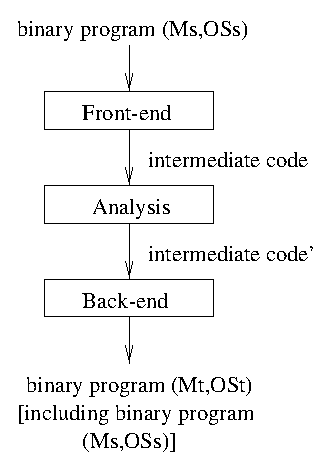
\includegraphics{figures/static.eps}}
\centerfigend{fig-static}{Structure of a static binary translator for
	source machine $M_s$, target machine $M_t$, source operating system
    $OS_s$ and target operating system $OS_t$.}
 
The fallback mechanism used by static binary translators is a runtime
environment that completely supports the source platform, and
hence includes an interpreter for source machine instructions, and support
for translation and mapping of operating system calls into the new
platform.  The development of a runtime environment is a significant
overhead; especially the mapping of operating system calls.  There is
little performance data reported in the literature regarding the amount of
time spent by binary translated applications in the interpreter mode.
Code ported from a proprietary CISC to RISC machine at Tandem, where the
operating system was binary translated to the new machine, reports an
average figure of 1\% of the time being spent on interpretation~\cite{Andr92}.
Informal talks with people who have developed such translators state that
the interpretation mode is seldom used if you have sufficient coverage 
of the patterns generated by compilers commonly used in that platform. 
Existing static translators have dealt mainly with procedural code, 
rather than object-oriented code, which poses new limitations to static
translation due to their dynamic nature of code dispatching through 
vtables.  
 
 
\subsection{Dynamic binary translator}
A dynamic binary translator performs the translation of the code while 
the program is being executed by the translator; that is, the input 
binary program is dynamically analyzed and translated into the target 
machine code during runtime.
Dynamic translation techniques overcome some of the shortages of static
translation, for example, determining the targets of indirect jumps.
Dynamic translation is able to support most practical cases of 
self-modifying code; code normally not supported in static translations.
Given that all the processing of a dynamic translator is done ``on the
fly'', the types of optimizations and analyzes have to be carefully
considered and optimized so that the minimum amount of time is spent
during runtime.
 
The structure of a dynamic binary translator is depicted in
Figure~\ref{fig-dynamic}\footnote{
Figure~\ref{fig-dynamic} by the SELF team at Sun Microsystems Labs.}.  
The binary program is fed into the front end which generates an 
intermediate representation for a block of code.  This representation 
is then compiled or emulated by the translator to generate
(unoptimized) machine code for the target machine.  If at any time the
translator determines that a new region of the program needs to be decoded,
the front end is dynamically invoked to parse that region and provide the
intermediate representation.  When generating machine code, counters are
kept on the number of times blocks of code are executed; once a threshold is
reached, machine code is regenerated to produce better machine code---this
process can be repeated several times, hence producing better code on a
demand-driven basis.  It is important to note that the translation is done
in a lazy fashion; that is, code is only translated when its path is reached.
In this way, fragments of the program that are not executed during runtime,
are not translated either.  Self-modifying code is handled by
invalidating the existing intermediate representation and re-parsing
the binary code with the changed bytes.
 
\centerfigbegin
\resizebox{!}{6cm}
{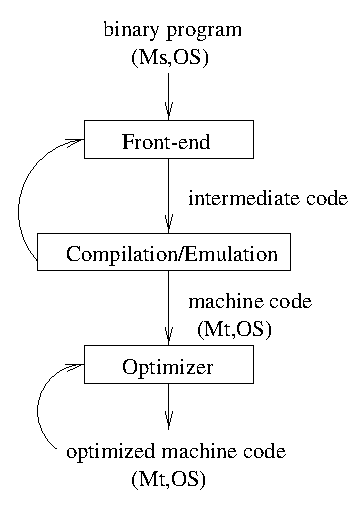
\includegraphics{figures/dynamic.eps}}
\centerfigend{fig-dynamic}{Structure of a dynamic binary translator for
    a source machine Ms, a target machine Mt and a multi-platform
    operating system OS.}
 
Dynamic compilers can perform runtime optimizations of the code based
on the execution profile of the program, hence several optimizations,
such as dynamically-dispatched calls and procedure inlining, can only be
possibly done on a dynamic compiler rather than using static techniques.
The performance penalty of code generated by such a translator is estimated
between 0.9X to 2.4X times that of code generated by a native optimizer
C++ compiler (these figures are based on code generated by the SELF-93 dynamic
compiler~\cite{Holz95}).
 
An interesting point to note is that a dynamic binary translator for
a multi-platform operating system does not require the development of
a runtime environment to support the mapping of old operating system
calls, as all translations are done ``on the fly''.  Using static techniques
in this case will still require a runtime environment to cater for the
interpretation of old machine instructions--dynamic techniques alleviate
the need for this fallback mechanism, but compromise the speed of 
execution of the program at the expense of less analysis and code
quality.
 


